\documentclass[11pt]{article}

\usepackage[a4paper]{geometry}
\geometry{left=2.0cm,right=2.0cm,top=2.5cm,bottom=2.5cm}

\usepackage{ctex}
\usepackage{amsmath,amsfonts,graphicx,amssymb,bm,amsthm}
\usepackage{algorithm,algorithmicx}
\usepackage[noend]{algpseudocode}
\usepackage{fancyhdr}
\usepackage{graphicx}
\usepackage{listings}
\usepackage{makecell}
\usepackage{titlesec}
\usepackage{hyperref}

\renewcommand{\emph}[1]{\begin{kaishu}#1\end{kaishu}}

% 设置一级标题格式
\titleformat{\section}{\normalfont\Large\bfseries\center}{\thesection}{1em}{}

% 设置二级标题格式
\titleformat{\subsection}{\normalfont\large\bfseries}{\thesubsection}{1em}{}

% 设置三级标题格式
\titleformat{\subsubsection}{\normalfont\normalsize\bfseries}{\thesubsubsection}{1em}{}


\newcommand\E{\mathbb{E}}

\begin{document}

\begin{titlepage}
    \vspace*{\stretch{1}}
    \centering
    \Huge\bfseries 机器学习汇报\\
    \huge 多模态会话情感分析\\
    \mdseries
    \vspace*{\stretch{2}}
    \large
    \begin{tabular}{l}
        {姓名:马迪峰}
        {学号:}\\
        {姓名:盛子轩}
        {学号:}\\
        {姓名:贾城昊}
        {学号:2021K8009929010}\\
        {姓名:李金明}
        {学号:2021K8009929016}\\
        {姓名:牛浩宇}
        {学号:2021K8009929007}\\
    \end{tabular}
\end{titlepage}

\tableofcontents

\newpage


    \section{题目说明}
    通过多模态数据(音频、文本、视频等)对会话情绪进行识别。利用给定的特征数据集,
    通过对三种模态数据的融合,建立稳定的情感识别模型,预测出会话时的情绪状态,
    包括happy, sad, neutral, angry, excited or frustrated六种情绪类别。


    \section{背景介绍}
    随着社交媒体分析、心理医疗、智能客服等行业的快速发展,用户的情感体验成为这些领域关注的焦点。
    传统的情感分析方法主要依靠人工标注、规则设计等方式获取特征,并结合机器学习算法进行分类。
    然而,这样的方法存在数据集小、适用性差、泛化能力弱等问题,难以应对多变复杂的应用场景。
    为了获得更好的性能,融合不同模态的方法至关重要。

    多模态情感识别的研究在人机交互、人工智能等领域有着重要的研究意义,备受研究者关注。
    在客户服务、智慧医疗、心理健康等领域具有广泛的实际应用价值。如何通过人类情感相关的语音、
    视觉、文本等数据准确识别人的情感状态,不同模态信息的融合方法至关重要。为促进多模态情感识别研究的进一步发展,
    推动该技术在实际应用中的落地和普及,实现更加精准、全面和智能的情感分析,需要建立有效稳定的情绪识别模型。
    相关工作将帮助社交媒体、客服中心、在线教育等领域的企业及机构更好地理解和满足用户需求,提高用户满意度和忠诚度。

    举例说明:假设一个会话场景为一个病人正在和心理医生进行远程心理治疗视频,他们会通过视频图像、
    语音和文本聊天三种数据形式进行交流。如果其中医生说到了一件让病人感到悲伤的事情,那么病人的语音音调、
    面部表情以及聊天内容等都可能会发生变化,这些变化就可以被用来推测出该会话的情绪状态。
    心理医生通过病人情绪状态的反馈,及时调整谈话内容,帮助病人缓解负面情绪,找到适合的治疗方法。


    \section{问题分析}
    多模态情感分析涉及到不同类型的数据,文本、图像、音频等。这些数据之间的异构性使得模型需要能够处理不同模态之间的关联,
    一方面模型需要学习如何有效地表示和概括来自不同模态的信息,另一方面需要将多模态的数据进行融合,连接多种模态的信息,
    从而完成推理。如果当中一种模态数据丢失时,不同模态的信息在推理中具有不同的预测能力和噪声拓扑,并且在不同模态、
    表示、预测模型之间进行知识迁移。

    在多模态学习中,最困难的部分在于多异构数据如何结合,不同级别的噪声如何处理,丢失数据如何处理。
    对于多模态情感分析任务,难点还在于如何将建模多种不同形式的数据之间的相互关系,最终得出准确的情绪识别结果。


    \section{典型方法}
    
    如今的情感分析研究通常采用深度神经网络,并专注于对上下文和说话人敏感的依赖关系进行建模。根据是否利用说话人信息,
    现有的方法可以分为两类:不考虑说话人的方法和依赖说话人的方法。

    不了解说话者的方法不能区分说话者,只注重捕捉对话中的上下文信息。HiGRU包含两个门控循环单元(gru),
    分别用于模拟单词和话语之间的上下文关系。AGHMN使用分层记忆网络来增强话语表征,并引入注意GRU来建模上下文信息。
    MVN 利用一个多视图网络来模拟对话中的词级和话语级依赖。
    
    相反,依赖于说话人的方法既对上下文敏感,也对说话人敏感。DialgueRNN利用三种不同的\\GRU分别更新对话中的说话人、
    上下文和情绪状态。DialgueGCN使用图卷积网络对说话人和对话顺序信息进行建模。HiTrans由两个层次转换器组成,
    用于捕捉全局上下文信息,并利用一个辅助任务来建模说话人敏感的依赖关系。然而,它们大多是针对语篇情态而提出的,
    而忽略了其他情态的有效性。
    
    
    \section{数据集介绍}

    IEMOCAP(Interactive Emotional Dyadic Motion Capture)是一个常用的情绪识别研究数据集,
    其目标是为多模态情感识别提供一个资源丰富、真实生动的数据集,以实现情绪在交互式对话中的自然表达和识别。

    数据集主要基于采集到的大量脸部动作捕捉、音频和文本记录。该数据集包含来自10对演员(5\\男5女)
    进行的大约12小时的自然面对面对话,并分成了151段对话。每段对话都有所对应的ID标识符、每段对话的男女对话顺序、
    每段对话里面的对话句子文本特征、音频特征和该对话句子所对应说话者的脸部图像特征以及真实的情感标签。

    这些对话场景包括了两人的合作任务、角色扮演和自由聊天等情境。参与者在对话期间佩戴了高精度的面部表情捕捉设备,
    还通过麦克风录制音频,同时记录下了他们的文本转录。

    IEMOCAP数据集中每种特征已经预处理为了python二进制保存(.pkl)的字典类型,字典的键是对话的标签(label),
    其对应的值是一个列表,该列表的长度是不固定的,列表中的每个元素是一个固定维度的numpy数据,
    该numpy数组即是一句对话的特征值,其中文本特征为1024维,图像特征为1582维,音频特征为342维。
    列表的长度即为每段对话中句子数量,Speakers.pkl记录了每句对话说话对象,train\_label则是对应每个句子的标签值。
    
    以下是对本题目所给数据集文件的具体说明:
    \begin{center}
        \begin{tabular}{|c|c|c|}
            \hline
            \textbf{文件类型} & \textbf{文件名} & \textbf{备注} \\
            \hline
            训练集 & train\_ids.csv & 训练样本对话的ID\\
            \hline
            测试集 & test\_ids.csv & 测试样本对话的ID\\
            \hline
            数据文件 & text\_features.pkl & 所有对话的文本特征\\
            \hline
            数据文件 & audio\_features.pkl & 所有对话的音频特征\\
            \hline
            数据文件 & visual\_features.pkl & 所有对话的图像特征\\
            \hline
            数据文件 & IDs.pkl & 每个对话的ID\\
            \hline
            数据文件 & train\_label.pkl & 训练样本对话中对话句子的真实标签\\
            \hline
            数据文件 & Speakers.pkl & 所有对话中男女人物对话的顺序,M代表男性,F代表女性\\
            \hline
        \end{tabular}     
    \end{center}


    \section{解决方法}
        \subsection{传统机器学习(集成学习)模型}
            \subsubsection{设计思路}
            我们小组大作业通过传统方法与深度学习方法两种途径实现文本的情感分析。
            传统方法与深度学习都有各自的特点,以下是两种方法在情感分析方面所采用的大致流程:
            
            传统方法主要基于手工提取文本特征,如词袋模型、TF-IDF等,然后将这些特征输入到朴素贝叶斯、
            支持向量机等传统算法中进行分类。深度学习方法则是将文本数据直接输入到神经网络中,
            通过训练得到特征和模型。
            
            深度学习模型可以自动学习文本中的特征,包括词汇的上下文、语法结构等。
            这使得模型能够更好地理解文本内容,从而获得更高的分类和情感分析性能。此外,
            深度学习模型通过训练可以不断优化自身,使得模型性能不断提高。
            
            在机器学习的有监督学习算法中,我们的目标是学习出一个稳定的且在各个方面表现都较好的模型,
            但实际情况往往不这么理想,有时只能得到多个有偏好的模型(弱监督模型,在某些方面表现的比较好)。
            集成学习就是组合这里的多个弱监督模型以期得到一个更好更全面的强监督模型,
            集成学习潜在的思想是即便某一个弱分类器得到了错误的预测,其他的弱分类器也可以将错误纠正回来。
            单个学习器我们称为弱学习器,相对的集成学习则是强学习器。
            
            我们小组大作业中所采用的集成学习模型是基于训练出的多个弱的基学习器,
            在此之上使用\\adaboost实现boosting算法以及使用
            bagging算法,通过对弱基学习器的训练不断做强化以及最后基于bagging实现加权平均算法的得到结果。
            
            选择集成学习模型最大的原因是想通过传统机器学习方法进行训练从而形成深度学习方法的对照组。
            同时由于单个的决策树,逻辑斯蒂回归等训练出的基学习器的预测结果难以令人满意,
            因此考虑通过集成学习的方法来提升训练的效果。
            
            优缺点:基于传统机器学习的情感分类方法主要在于情感特征的提取以及分类器的组合选择,
            不同分类器的组合选择对情感分析的结果有存在一定的影响,
            这类方法在对文本内容进行情感分析时常常不能充分利用上下文文本的语境信息,
            存在忽略上下文语义的问题,因此其分类准确性有一定的影响。


            \subsubsection{算法流程}
            集成学习模型首先基于决策树,随机森林或逻辑斯蒂回归来生成基学习器。在基学习器的生成过程中使用了adaboost算法。
            由于一共有151段对话,且bagging算法较为注重各个基学习器之间的独立性,
            希望每个基学习器能基于自己的训练数据给出自己相对独立的预测结果。因此在分配训练数据的过程中,
            会根据对话集来分配不同基学习器的训练数据。后由于单独的一个对话集训练数据过少导致容易过拟合,且泛化性能很差,
            因此尝试对每个基学习器的训练数据随机分配3-4个对话集进行训练。
            \begin{center}
                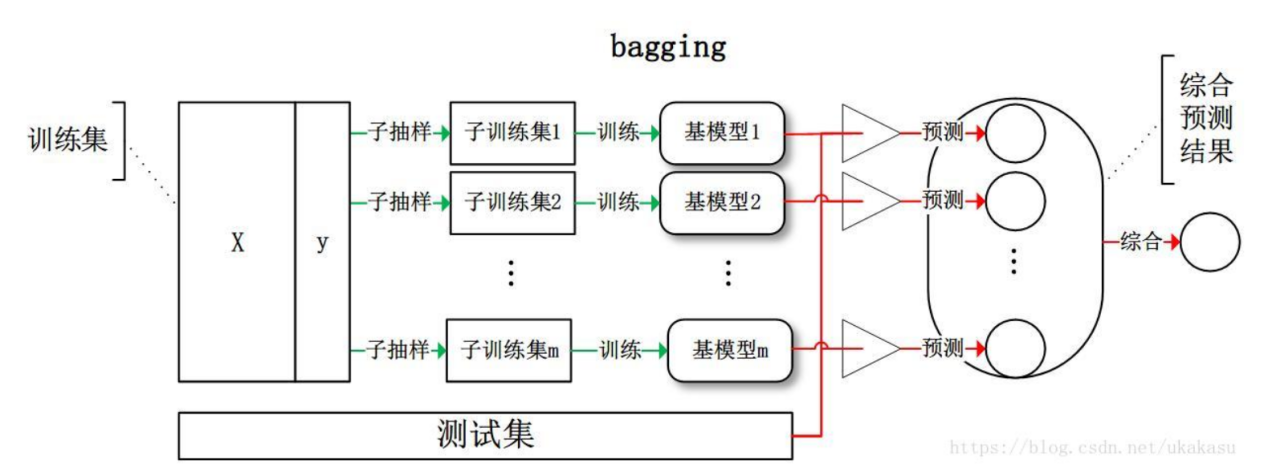
\includegraphics[scale = 1.1]{graph/tradition1.png}
            \end{center}

            在基学习器的训练过程中,会使用adaboost算法进行迭代,迭代三次来获得不同的基学习器,
            每次根据上次训练出的基学习器在训练集上的误差来进行训练数据的权重分配一进行迭代
            (具体实现可以参考adaboost算法以及代码实现)。
            \begin{center}
                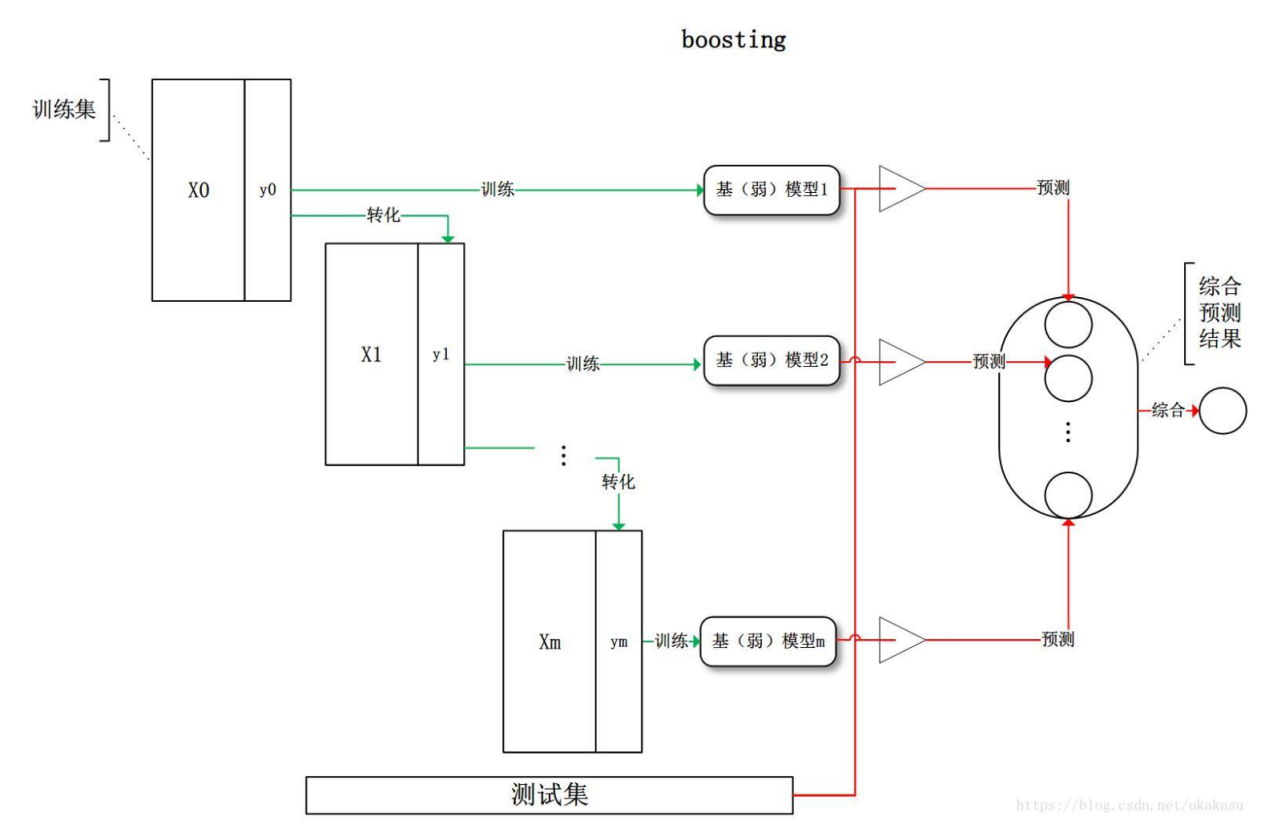
\includegraphics[scale = 1.1]{graph/tradition2.png}
            \end{center}

            在训练完成151个基学习器之后,并不会立刻进行预测并进行众数选举,而是会让每个基学习器在整个的训练集上进行预测来确定其泛化性能,
            并根据其预测的正确率来判定其最终投票的权重,实现bagging算法中的加权平均算法。

            由于传统学习方法中不能对文本音频图像三个特征矩阵进行整合,因此上述的训练过程均是基于单个方面进行训练,
            最终还需由三个学习器进行投票得到最终的结果。最终训练效果不尽人意,但相比随机猜测的正确率确实有较为显著的提升。



            \subsubsection{调整与改进}
            \begin{enumerate}
                \item [1.]在设计的过程中,曾遇到过如何使用集成学习的方法。一种可能的情况是直接使用随机森林,
                        不考虑151个对话集之间的独立性而直接在所有的对话上分割训练集进行训练。
                        但如此训练后发现效果不尽人意,与不采用集成学习方法的效果相差无几,
                        因此产生了通过对话集来进行训练数据的分割并训练基学习器的想法,
                        通过此种方法也能在传统机器学习的框架下更好的去兼顾上下文,
                        从而使得基学习器的预测数据相对更为独立和准确。
                        事实证明采用这种方法后预测准确率提升了7个百分点。
                \item [2.]通过后来的逐步实践发现,只采用一个对话集训练一个基学习器的训练数据过少,
                        查看基学习器的预测数据发现效果仍不太好,因此在根据不同的对话集进行训练的基础上,
                        通过随机添加对话集的方法,将每一个基学习器的训练数据增加到4个对话集,
                        这种方法增加每个基学习器的泛化性,使其效果有所提升。
                \item [3.]通过上述的方法,已经基本完成了bagging的相关方法的应用,但阅读课本与查阅资料,
                        了解到通常可以将boosting方法与bagging方法混用,以此来进一步提高其预测准确率。
                        在每个基学习器的训练过程中,考虑到根据以上方法的训练,
                        每一个基学习器的预测性能还可以进行加强,为了对弱的基学习器进行强化,采用adaboost算法,
                        每一次训练后根据错误率对样本进行加权,多次训练强化基学习器,其效果也是显著的。
                \item [4.]在通过bagging训练完后,该如何对151个基学习器的预测结果进行投票选举呢?
                        这也曾是一个让我困惑的问题。我最开始采用的是平凡的方法,通过众数进行简单的投票选举。
                        但后来我改进了想法,决定首先在训练集上进行预测来获得权重,由此来进行加权平均法。
                        此种方法下,最终的投票结果会根据每个基学习器的权重在每个结果上的相加,
                        然后比较权重大小来得到最终的预测结果。
            \end{enumerate}

            \subsubsection{对问题和模型的理解}
            多模态情感会话分析是指通过结合多种媒体形式(如文本、图像、音频、视频等)来分析和理解会话中的情感信息。
            它是多模态情感分析的一个重要研究方向。在我们的大作业中,其具体体现为每一个句子拥有文本,音频,
            图像三个特征,分别对应了1024位,342位,1582位的特征向量。

            多模态情感分析的一大重点在于需要对上下文进行充分的理解。在训练的过程中对这个特性我进行了大量的思考,
            其中最大的改进就是放弃了直接在所有对话上采用随机森林的做法,而是认为的根据对话集进行划分来进行训练。
            虽然传统方法中很难在本质上做到对上下文的兼顾,但考虑了这个特性之后的训练结果相比直接的随机森林确实有不小的提升。

        \subsection{LSTM模型}
            \subsubsection{模型简介}
            神经网络分为两种,前馈型神经网络与后馈型神经网络(即递归型神经网络);前馈型神经网络典型的有:
            卷积神经网络(Convolutional Neural Networks,CNN);后馈型(递归型)神经网络的典型有:
            循环神经网络(Recurrent Neural Network)
            
            前馈神经网络(Feedforward Neural Network,缩写为FNN)是一类最简单的神经网络,
            也是最早出现的神经网络之一。它主要由若干层神经元组成,各层神经元之间没有反馈连接,
            信息只能向前流动,从而得名“前馈”。通常,输入层负责接收原始数据,
            中间隐藏层则对数据进行一系列非线性映射和特征提取,输出层则产生神经网络的输出结果。
            
            反馈神经网络(Recurrent Neural Network,缩写为RNN),具备反馈(或循环)连接,
            即输出可以在后续的时间步骤被送回给网络的输入端。这种机制使得RNN能够处理那些需要记忆和上下文信息的复杂任务,
            例如语音识别、机器翻译、自然语言理解等。然而,由于反馈神经网络的训练相对较为复杂,
            容易产生梯度消失和爆炸等问题,因此虽然RNN在某些场合具备优势,但并不是适用于所有的神经网络任务。
            
            对于普通的前馈神经网络,神经网络会认为我们 $t$ 时刻输入的内容与 $t+1$ 时刻输入的内容完全无关,显然,
            这样的考虑在众多应用场景中是不存在问题的,例如图片分类识别。然而,对于另外一些情景,例如自然语言处理 
            (NLP, Natural Language Processing) ,合理运用 $t$ 或之前的输入来处理 $t+n$时刻显然可以更加合理的运用输入的信息。递归神经网络 (RNN, Recurssion Neural Network)就是被设计出来运用到时间维度上信息从而更加准确地在时间维度上处理数据,一个简单的递归神经网络可以用这种方式表示:
            
            \begin{center}
                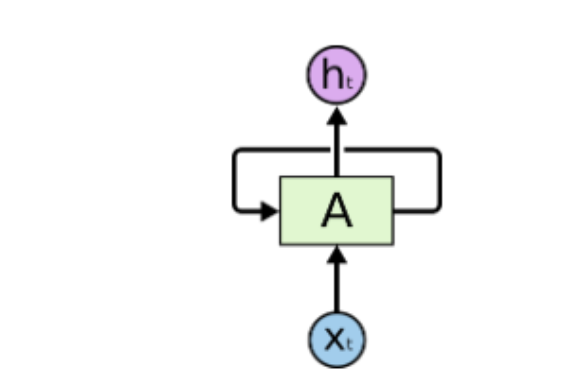
\includegraphics[scale = 0.7]{graph/lstm1.png}
            \end{center}

            在图中, $x_t$是在$t$时刻的输入信息, $h_t$是在$t$时刻的输出信息,
            可以看到神经元A会递归的调用自身并且将$t-1$时刻的信息传递给$t$时刻。具体来说,从多层网络出发到循环网络的思想来源是:
            在模型的不同部分共享参数。如果在每个时间点都有一个单独的参数,不但不能泛化到训练时没见过序列长度,
            也不能在时间上共享不同序列长度和不同位置的统计强度。循环神经网络在几个时间步内共享相同的权重,
            而时间步索引也不必是现实世界中流逝的实践,也可以表示序列中的位置。
            
            简单递归神经网络存在一个“硬伤“,长期依赖问题:由于变深的结构使得模型丧失了学习到先前信息的能力,
            从而让优化变得相当困难,循环网络要在很长的时间序列的各个时刻重复应用相同的操作来构建非常深的计算图,
            并且模型参数共享,这在量级过大的情况下会导致梯度消失和爆炸问题。
            
            LSTM,全称 Long Short Term Memory (长短期记忆) 是一种特殊的递归神经网络 。
            LSTM从被设计之初就被用于解决一般递归神经网络中普遍存在的长期依赖问题,该模型的核心贡献就是产生梯度长时间流动的路径,
            使用LSTM可以有效的传递和表达长时间序列中的信息并且不会导致长时间前的有用信息被遗忘,
            
            简单来说,LSTM的设计思想可以概况为:只有一部分的信息需要长期的记忆,而有的信息可以不记下来。
            LSTM循环网络“细胞”的框图可以表示为:

            \begin{center}
                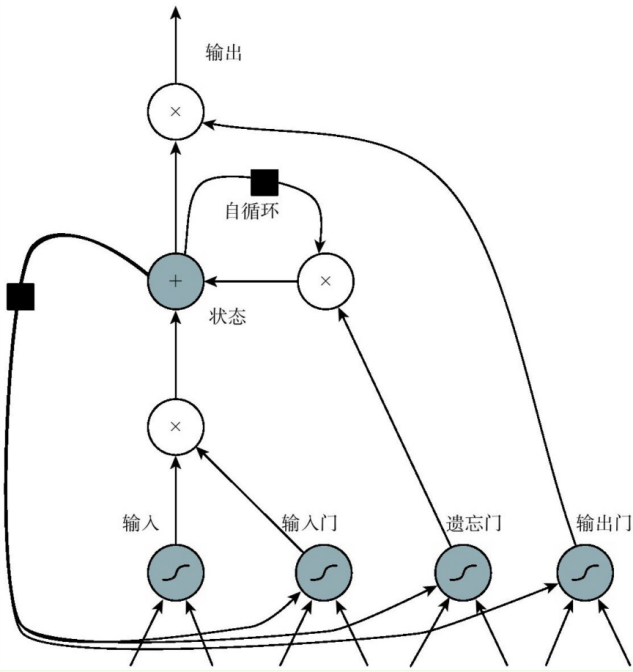
\includegraphics[scale = 1]{graph/lstm2.png}
            \end{center}

            细胞彼此连接,以代替一般循环网络中普通的隐藏单元。如果sigmoid输入门允许,它的值可以累加到状态。
            状态单元具有线性自循环,其权重由遗忘门控制。细胞的输出可以被输出门关闭。也就是说,
            LSTM是一种基于门控实现的网络结构。LSTM的关键是细胞状态,表示为$C_t$ ,
            用来保存当前LSTM的状态信息并传递到下一时刻的LSTM中,也就是RNN中那根“自循环”的箭头。
            当前的LSTM接收来自上一个时刻的细胞状态 $C_{t-1}$  ,并与当前LSTM接收的信号输入 $x_t$  
            共同作用产生当前LSTM的细胞状态 $C_t$ .

            \begin{center}
                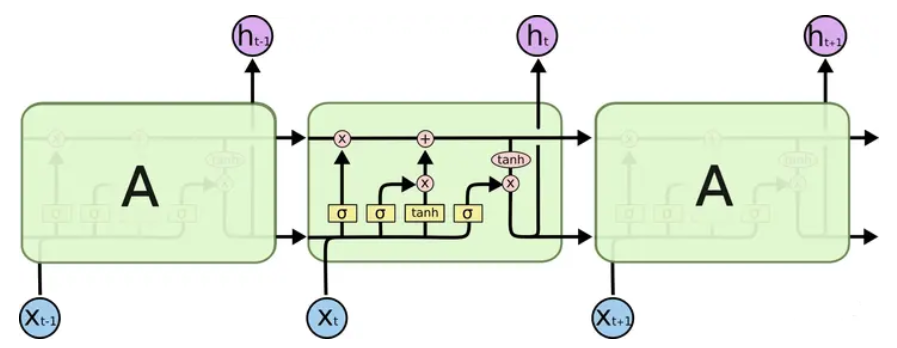
\includegraphics[scale = 0.6]{graph/lstm3.png}
            \end{center}

            总而言之,在决策树模型解决该问题接连碰壁后,在面对该多模态情感分析任务时,
            很自然想到利用LSTM处理序列数据的优良特性来尝试解决。这也是第二种方法我们选择LSTM的原因,
            但是很快后文也将提到,LSTM在面对该问题时依然会显得力不从心。


            \subsubsection{设计思路}
            那么怎么利用LSTM来对问题进行建模呢?这需要分析一下数据集的特征,前面已经提到,\\
            IEMOCAP数据集已经将各模态的特征预处理为了字典格式。
            简单的一个训练模型可以是一个\\LSTM层和一个全连接层,这个模型的参数包括四个,
            如input\_size(输入特征的数量)、hidden\_size(隐藏状态的大小)、num\_layers(LSTM层的数量)和num\_classes(输出类别的数量)。
            对于该多模态情感分析任务,每段对话可以被看作一个序列,每个句子是序列中的一个元素,
            句子的特征向量就是元素的值。每个时间步长输入到LSTM单元的特征数量即我们对应的每种模态句子的维度数量。
            例如,如果是处理数据集中的文本序列,input\_size就是文本句子向量的维度。
            具体的训练过程如下:
            \begin{enumerate}
                \item [1. ]
                定义模型:使用句子特征向量的维度作为input\_size,选择一个合适的hidden\_size和num\_layers,
                并将num\_classes设置为6(共6种情感类型)

                \item [2. ]
                定义损失函数和优化器:对于分类问题,通常使用交叉熵损失函数。优化器可以选择Adam。

                \item [3. ]
                训练模型:对于每个epoch,对于每段对话,将对话和对应的情感标签输入到模型中,
                计算输出和标签之间的损失,然后反向传播误差并更新模型的参数。

                \item [4. ]
                验证模型:在验证集上评估模型的性能,调整模型的参数或训练过程以优化性能。

                \item [5. ]
                测试模型:最后,在测试集上评估模型的性能。

            \end{enumerate}
            
            注意:在实际操作中,需要对数据进行一些预处理,因为每段对话的句子特征向量的长度不同(句子个数不同),
            需要使用填充(padding)或截断(truncation)来使它们的长度相同。为了在\\CUDA上进行训练,
            还需要将数据和标签转换为PyTorch的Tensor格式,并转移到CUDA上。
            
            为了在训练LSTM模型时体现一段对话内句子的上下文相关性,应该将整个对话作为一个序列输入到模型中,
            从而LSTM模型可以处理序列数据,并且在处理每个元素时都会考虑到前面元素的信息。
            
            在每个epoch中,遍历对话数据集,对于每个对话,将对话中的所有句子特征向量按照它们在对话中出现的顺序组成一个序列,
            然后将这个序列输入到模型中。标签也应该是一个与序列长度相同的标签序列,
            其中每个标签对应于序列中相应句子的情感分类。
            
            最后训练出来的结果的每个句子对应的特征是一个6维向量,该向量的每个值是取对应标签的概率,
            这是在做多分类任务时常用的方法和手段,最后调用python的argmax方法即可取到最终的结果。
            
            \subsubsection{优化和改进}
            \begin{enumerate}
                \setlength{\parindent}{2em}
                \item [1. ]\textbf{初步尝试}\par
                GRU(Gate Recurrent Unit)是循环神经网络(Recurrent Neural Network, RNN)的一种,
                和LSTM(Long-Short Term Memory)一样,也是为了解决长期记忆和反向传播中的梯度等问题而提出来的。
                GRU和LSTM的区别主要体现在,GRU的形式更为简洁,参数较少,计算效率更高,
                在某些情况下会忽略一些长程信息,在该情境下,直接使用两种模型的效果是差不多等效的,都很烂。
                
                如果直接用单独的模型训练,且只使用一种模态的信息,发现无论是测试集还是训练集,正确率都会很低,
                只比一开始决策树的效果好一点,差不多是15-17\%。猜测就是因为此时模型的表达能力还不够,因此需要增加一些层数。
                
                \item [2. ]\textbf{再次尝试}\par
                为了增加模型的复杂度和可表达性,我们尝试在LSTM后增加了线性层、卷积层等,但是依然存在梯度消失的问题,
                于是我们引入了残差层,残差连接技巧主要用于深度神经网络的训练中,尤其是在深度网络层数较多时。具体而言,
                残差连接技巧可以通过跨层直接连接来提供捷径,从而缓解梯度消失问题,增加模型的深度,从而提高模型的表达能力和性能。
                由于残差连接可以提供跨层直接连接的效果因此可以使模型更容易收敛,减少训练时间和计算资源的消耗。
                \begin{center}
                    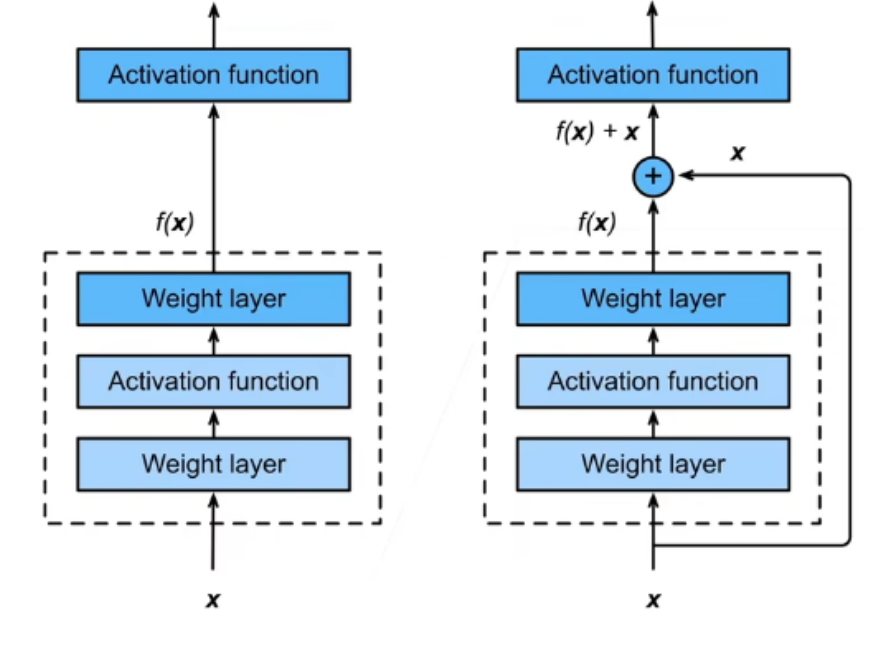
\includegraphics[scale = 1]{graph/lstm4.png}
                \end{center}

                增加模型复杂度后,确实在loss的收敛上和测试集正确率上有了比较好的表现,但是仍然不能算是一个可用的模型,因为效果还是很差。
                
                一开始我们怀疑是过拟合导致泛化性能比较低,因此还引入了正则化层来缓解,但是发现并没有产生什么很大的变化。
                为了继续改进基于LSTM的模型效果,我们又尝试引入了多种模态的效果。


                \item [3. ]\textbf{最终妥协}\par
                最后我们还是决定将多种模态的信息融合送入模型,来查看是否结果是与模态
                种类和特征是强相关的,所以我们将每个模态通过一个LSTM,将结果合起来后通过一个线性层送出,
                并且引入了一种多模态的门控处理,这样进行处理后,模型的性能在测试集上确实有所提升,
                但是泛化性能并没有提高很多。
                
                另一方面,我们意识到当前模型显然是已经存在梯度消失的现象,loss无法进一步下降,
                所以可能是找到了一个局部最优的区域。最后我们又尝试引入了模型的参数初始化方法,
                对模型的中的各种层的参数进行初始化,并且将单向LSTM改成了双向LSTM ,再次改进后,
                效果确实已经达到了历来的最好。loss成功降到了0.35附近,训练集正确率能够达到45\%,
                测试集也成功达到了25\%的效果,说明改进确实是有效果的。并且loss已经成为了一个扰动极小的值,
                但是正确率依然无法进一步提高,那就足以说明,即便是做了种种尝试,该模型的表达能力还是不足以完成任务,
                它无法学到ground truth对应的函数关系,因此我们只好放弃LSTM,寻求更有效的模型进行训练。

            \end{enumerate}

        \subsection{Transformer\_Based模型}
            \subsubsection{模型简介}
            我们使用了一种基于Transformer编码器的模型,综合考虑数据集中的三种特征,文本、音频和图像。
            具体来说就是在模态编码器中引入模态内和模态间的Transformer编码器来捕获模态内和模态间的相互作用,
            并将位置和说话人嵌入作为这些Transformer编码器的额外输入来捕获上下文和说话人性别的信息。
            
            在提取了话语级单模态特征后,Transformer\_Based模型设计了9个捕获模态内和模态间交互的模态编码器,
            并借鉴GRU的门控机制对输出进行处理,并拼接后通过一个线性层,得到每个模块的输出信息。
            
            然后我们通过一种分层门控融合策略,动态融合来自多种模态的信息。最后,通过一个线性映射,
            将每个模态的输出和融合后的分别输出映射到类别维度,后者用于得到预测情感的label,
            前者则与后者一起参与loss的计算。
            
            为了综合评估每轮的训练结果,我们设计了一种损失来全面考虑每个模态的预测和最终结果的预测,
            以学习更好的模态表示。
            
            总体设计图如下:
            
            Ljm to do:画图
            
            \subsubsection{Transformer编码器层简介}
            Transformer 模型的编码器层是该模型的关键组件之一,它负责处理输入序列的信息并生成表\\示。

            \begin{center}
                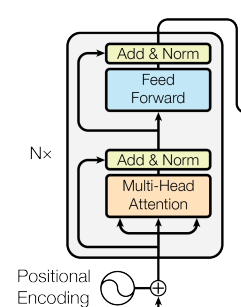
\includegraphics[scale=0.9]{graph/transformer1.png}
            \end{center}

            下面是其关键组件:
            \begin{enumerate}
                \setlength{\parindent}{2em}
                \item [1. ]\textbf{多头自注意力机制}\par
                自注意力机制允许模型在处理序列时分配不同的注意力权重给序列中的不同位置。对于输入序列的每个位置,
                模型计算出一个权重向量(通过Q,K,V矩阵),用于加权组合所有位置的信息。
                这使得模型能够在处理序列时更好地捕捉上下文信息。

                为了增强模型对不同位置和不同关注方向的建模能力,自注意力机制被扩展为多头注意力机制。
                在多头注意力中,模型计算多组注意力权重,每组权重被称为一个“头”。
                这些头的输出被拼接在一起并通过线性变换进行整合。

                \begin{center}
                    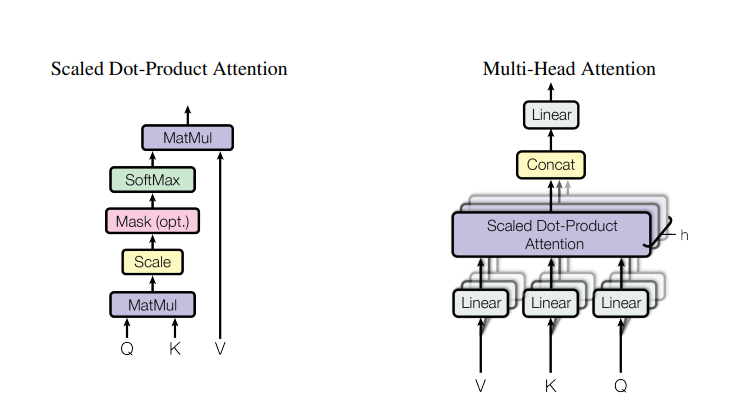
\includegraphics[scale=0.9]{graph/transformer2.png}
                \end{center}

                \item [2. ]\textbf{前馈神经网络}\par
                编码器层的每个自注意力子层后都连接着一个前馈神经网络。前馈神经网络是一个全连接的前馈结构,
                它对自注意力子层的输出进行非线性变换。这有助于模型学习更复杂的序列特征表示。

                \item [3. ]\textbf{残差连接和层归一化}\par
                在每个子层(自注意力和前馈神经网络)的输入和输出之间都有一个残差连接。这有助于防止梯度消失问题,
                并使得更容易学习恒等映射。层归一化用于规范每个子层的输出,提高训练稳定性。

                \item [4. ]\textbf{位置编码}\par
                Transformer 模型不包含序列顺序信息,因此为了使模型能够处理序列,通常会在输入中添加位置编码。
                位置编码是一种用于表示单词或序列位置的向量,通过将这些位置编码添加到输入中,
                模型可以区分序列中不同位置的单词。


            \end{enumerate}

            \subsubsection{建模与改进过程}
            \begin{enumerate}
                \setlength{\parindent}{2em}
                \item [1. ]\textbf{最初尝试:直接复用Transformer}\par
                在LSTM效果不好后,我们很自然地想到用Transformer进行建模。在对LSTM的loss进行分析,我们认为LSTM失败的原因是其表达能力不够,
                而且很容易出现梯度消失的问题(即在训练50轮后loss便基本不再下降,但此时在训练集上的正确率只有40\%),
                为了缓解这个问题,我们尝试加上残差连接等一系列操作,但效果仍然不好,最后决定放弃LSTM,尝试使用Trans-former进行建模。
                除了模型的表达能力外,Transformer的训练时并行的,即所有字是同时训练的。而LSTM的训练是迭代的、串行的,
                必须要等当前字处理完,才可以处理下一个字。这样就大大增加了计算效率。
                
                但是,过程却并没有特别顺利,Transformer模型最初是用于处理NLP的问题,而不是用来分类,
                所以其编码器-解码器模型架构下,需要使用起始符和终止符来判断输出是否结束。但是对于我们的问题来说,
                输出的维度是确定的,而且数据集给定的特征是经过了处理了的,所以没有办法得到一个好的起始符和终止符的表达。
                
                按照Transformer的论文的做法,训练时会把预期的输出结果传入解码层进行训练,于是本组成员最初也把训练集的标签作为输入传入了解码器,
                然后很快训练集的正确率便到达了\\100\%。但是应用到测试集时,由于没有起始符的编码,我们最初使用全0作为起始符,
                但很显然,最终测试集的结果很差。最后查看预测结果发现,预测的都是同一个类型,在通过分析后,
                我们意识到这是因为模型学习到了从label到预测输出的恒等映射,所以当预测没有label输入后,
                其预测结果完全根据输入的没有含义的起始符而不是输入信息。

                在之后,我们尝试了在训练时也加入自定义的起始符和终止符用作输入,但这样操作后的模型在测试集的泛化能力仍然很差,
                甚至不如随即猜测。这让我们不得不思考直接复用Trans-former是否真的适合这个问题


                \item [2. ]\textbf{再次尝试:仅用编码层}\par
                鉴于上面的尝试,我们决定不使用Transformer的解码层,而只使用Transformer的编码器层,
                并把数据集的特征卷积后直接作为编码器层的输入,也不把label作为训练时的输入信息。
                这样既利用数据集的特征信息,也不用起始符和终止符的信息,而且避免了模型的预测受到\\label的影响。
                最重要的一点是,Transformer的精髓就在其编码器层,即多头自注意力机制,所以这样也能很好地捕捉对话序列中的前后联系,
                符合我们最初打算使用Transformer的想法。
                
                在这之后,本组的一个成员使用了Transformer编码器简单处理了文本特征,
                仅仅对输入特征进行线性映射到隐藏层的维度,然后通过Transformer的编码器,
                最后通过线性映射到6维(一共6个类别)。最后意外地发现,正确率达到了50\%左右,当然,
                此时模型的loss收敛速度较慢,但看到最终能达到50\%正确率之后,
                我们开始用Transformer对三个模态进行融合训练的尝试。
                
                \item [3. ]\textbf{改良模型:融合模型}\par
                
                融合多个模态是一个很复杂的问题,因为输入中不仅含有三个模态的特征,还包括说话人的性别。
                他们的形式各不相同,我们最初尝试直接拼接,但这显然不是一种好的处理方法。但各自训练得到输出后再综合考虑,
                又无法很好地考虑模态间的相互作用(至少前序的其它模态特征对当前的模态的特征的影响没有考虑),
                所以最后训练得到的模型泛化能力并不尽人意

                这之后我们意识到,如何融合视频,音频,文本三个模态是最重要的,也是先需要考虑的问题。
                经过讨论,我们发现Transformer模型的自注意力机制天然适用于模拟多模态间的相互作用。
                所以我们最终决定每两个模态的特征作为输入,处理后分别作为transformer编码层的Q和K,V,得到输出。
                这样一共会得到9个输出(一共三个模态,所以9个),下一步再把与每个模态有关的输出综合得到每个模态的最终输出,
                最后再综合这三个模态各自的输出,经过分类器降维后得到模型的最终输出。
                
                然后,需要考虑的是如何考虑说话人的性别,通过分析,说话人的性别与对话中语句的位置有很大的联系,
                所以在否定了多个方案后,最终我们在Transformer编码层输入前,除了加上位置编码,
                还加上了对说话人性别的信息。具体操作便是把性别映射成[0,1]或者[1,0],然后进行\\embbeding操作,
                加到输入信息中。
                
                最后便是对loss的考虑,其次我们只考虑最终的输出,使用交叉熵损失进行训练,
                此时正确率已经可以达到65\%左右,在一次偶然的讨论中,我们想到,
                可以综合考虑每个模态的输出和最终的输出,从而保证更好的预测,于是我们设计了一种计算loss的方式,
                综合考虑模态的预测和最终的预测,保证模态的输出结果本身更加可靠,最终也发现,
                这样设计后loss的收敛快了很多。

            \end{enumerate}
            \subsubsection{最终建模}
            所以,通过上面的探索过程,我们便得到了基于Transformer编码器的对于这个问题的建模,具体如下:
            \begin{enumerate}
                \setlength{\parindent}{2em}

                \item [1. ]\textbf{输入卷积}
                \par 在数据集中,文本,视频,音频的特征分别为1024,342,1582。
                为了确保三个模态的特征表示位于同一空间,我们将它们输入到一维卷积层中,
                保证输出的维度均为隐藏层的维度。
                
                \item [2. ]\textbf{位置嵌入}\par
                为了利用话语序列的位置和顺序信息,引入Transformer的位置嵌入来加上第一步得到的卷积输出

                其中pos为话语索引,i为维度索引。
                
                \item [3. ]\textbf{说话人性别嵌入}\par
                为了捕获话语序列中的说话人的性别信息,我们设计了说话人性别嵌入来加上第一步得到的卷积输出。
                说话人性别会在对话中被映射成一个向量:
                
                总体而言,通过第2、3步,我们将位置和说话人性别嵌入到了卷积层的输出。
                
                \item [4. ]\textbf{模态内和模态间的Transformer编码器:}\par
                我们用9个模态内和模态间的Transforner编码器来模拟三个输入模态内和模态间相互作用。
                Transforner编码器的多注意力层包含了三个输入张量:Q 、K、 V。对于模态内,Transforner编码器的Q、
                K、V张量均是该模态的输入信息;对于模态间,我们将一个模态的输入信息作为\\Transforner编码器的Q,
                另一个模态的输入信息作为Transforner编码器的K,V。

                通过上面操作,我们可以较好地模拟到对话中模态间的相互作用。
                
                \item [5. ]\textbf{门控机制}\par
                为了自适应地过滤掉输入的无关信息,我们借鉴了GRU的门控机制,设计了包含单模态和多模态的门控机制,
                以自适应地获得每个模态的预测输出,并分别动态学习这些输出之间的权重,最终得到最后的预测输出。
                
                我们首先使用门控制机更好地自适应选择Transformer编码器输出的相关信息。具体来说,
                首先将输入通过线性变换层后通过 Sigmoid 激活函数计算门控值 $z$。然后将将输入与门控值 $z$ 相乘,
                得到通过门控后的表示。接着,我们将与该模态有关的transformer的输出直接串联,
                最后通过一个全连通层后,得到该模态的最终输出。
                
                我们还设计了一种门控机制,使用softmax函数动态学习每个模态输出的权重。然后将权重与模态输出相乘,
                得到最终的综合了三个模态的输出。

                \item [6. ]\textbf{分类器}\par
                在得到上面三个模态融合的输出后,我们将输出通过一个线性映射,降维到6维(分类的种类为6),
                然后经过softmax层,得到每一个维度的概率。
                
                除此之外,我们还把每个模态的输出分别映射到6维,然后经过softmax层,用来计算每轮训练的loss。
                
                \item [7. ]\textbf{Loss计算}\par
                我们分别对最终融合了三个模态的输出和每个模态的输出进行交叉熵损失计算,并进行加权相加
                (这个权重需要自己定义,本次实验中均为1),得到最终的loss。
                
                Ljm to do: 添加公式

                
            \end{enumerate}

            \subsubsection{对问题的认识与思考}
            基于Transformer编码器的模型的泛化能力非常好,能达到70\%左右的正确率,相较于前面两种模型有了很大的提升,
            我们觉得一个重要原因是Transformer的具有很强的表达能力,且其自注意力机制,
            使得模型能够在不同位置关注输入序列的不同部分,更好地捕捉长距离依赖关。
            
            Transformer模型的结构天然适用于多模态输入(比如Q,K,V的机制),可以轻松地处理不同类型的输入数据,
            并模拟出不同模态之间的相互作用。所以,针对多个模态,Transformer\_Based模型综合地考虑了每个模态的信息,
            并且Loss的评估也综合考虑了每个模态的预测结果和总的预测结果,这使得其训练过程收敛很快,
            且预测的准确度较高。
            
            同时,为过滤掉Transformer编码层的无效信息,我们借鉴GRU的设计理念,添加了门控机制,
            这有助于模型选择性地更新和遗忘信息,从而更好地捕捉序列中与不同模态之间的依赖关系。
            并且在融合多个模态信息时,我们也设计了一种类似的门控机制,帮助模型自适应的学习各个模态的权重,
            提高了模型的学习和表达能力。
            
            除此之外,数据集的特征与标签也具有一定的区分性,这也是我们能得到较高泛化能力的前提,
            通过PCA降维画出来的数据分布如下:

            \begin{center}
                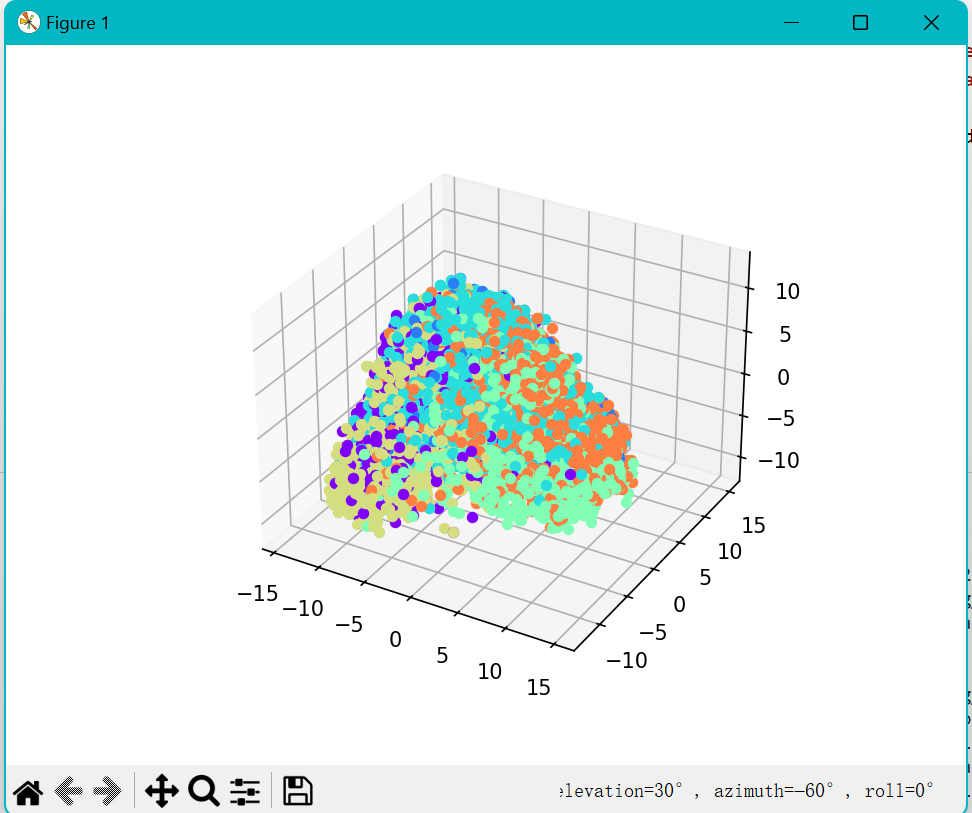
\includegraphics[scale=0.8]{graph/transformer3.png}\\
                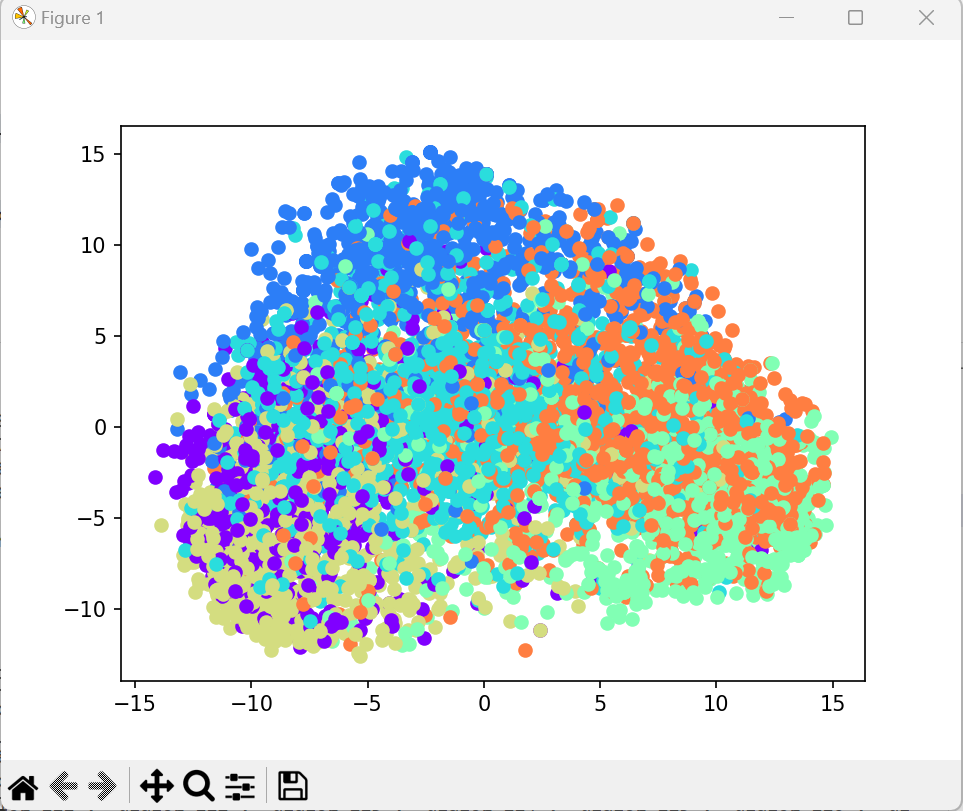
\includegraphics[scale=0.8]{graph/transformer4.png}
            \end{center}

            可以看到,即使降维之后,数据分布仍然具有一定的区分性,具体表现在不同颜色的数据集中的区域不同。

    \section{实验结果}
        \subsection{传统机器学习(集成学习)模型}
            \subsubsection{训练结果}
            \begin{enumerate}
                \item [1. ]\textbf{RandomForest做基学习器:20\%}
                \begin{center}
                    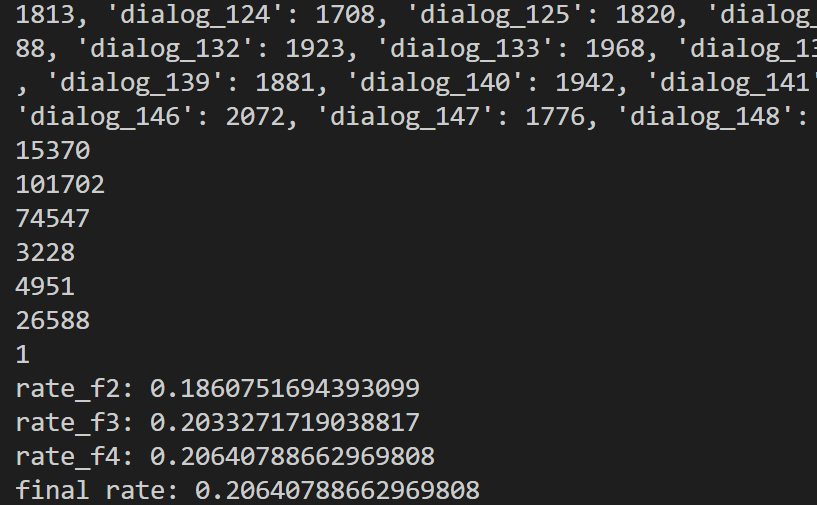
\includegraphics[scale=1]{graph/result1.png}
                \end{center}
                \item [2. ]\textbf{Decisiontree做基学习器:20\%}
                \begin{center}
                    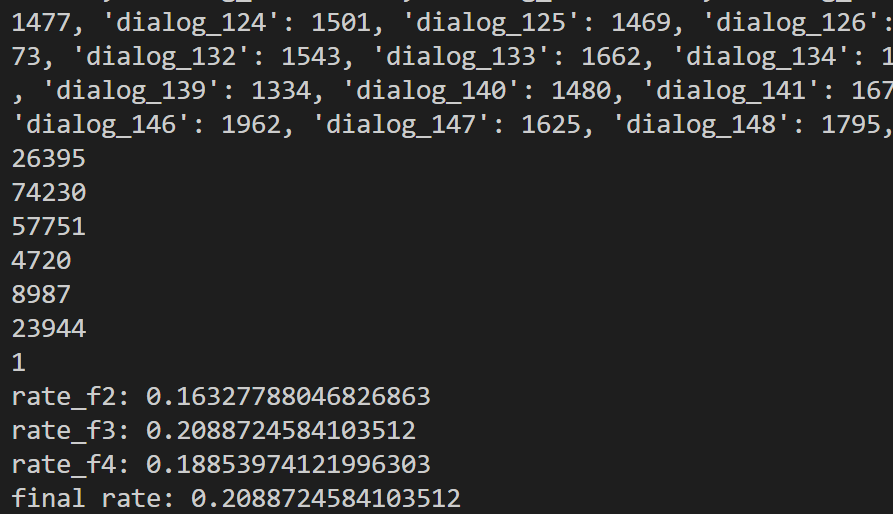
\includegraphics[scale=1]{graph/result2.png}
                \end{center}
                \item [3. ]\textbf{ogistic做基学习器:23\%}
                \begin{center}
                    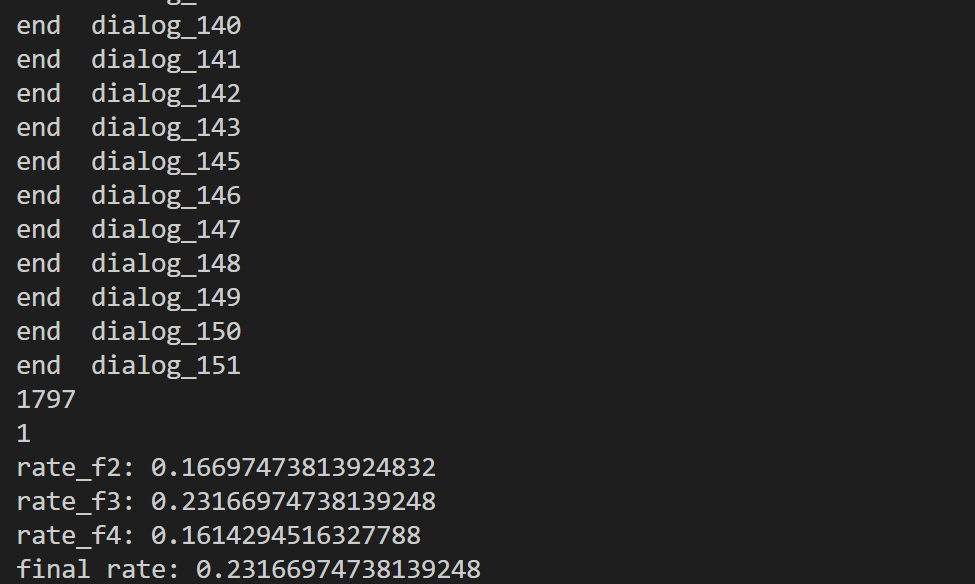
\includegraphics[scale=1]{graph/result3.png}
                \end{center}
            \end{enumerate}

            \subsubsection{结果分析}
            实践证明,传统机器学习集成学习方法在处理该问题时显得力不从心,
            
            在实践过程中我曾尝试过多种方法,并基本上运用了所有的集成学习的方法,
            但是最终的效果仍然难以达到使用transformer训练出的效果,可能的原因在于
            
            \begin{enumerate}
                \item [1. ]多模态情感会话分析需要考虑上下文,而Transformer模型的核心思想是自注意力机制,
                            能更好地理解序列中的上下文信息;相比之下传统学习方法往往是基于单个的语句进行训练,
                            并不能很好的兼顾整个对话的上下文,因此训练效果。

                \item [2. ]传统学习方法难以对多模态情感会话分析进行很好的建模。
                            在使用adaboost方法进行基学习器多次迭代的过程中发现,每一个基学习器再经过一轮训练后在训练数据上的预测效果往往惊人的好,
                            正确率可以达到90\%多(这也直接导致adaboost通过增加错误预测数据权重的多次迭代策略效果并不好),
                            但是泛化性能却非常差。造成这种现象的原因可能还是因为模型的建立本身存在一定的问题。
            \end{enumerate}

        \subsection{LSTM}
            \subsubsection{训练结果}
            准确率:17-25\%,改进后最高达到25\%
            
            
            实践证明,简单的LSTM模型在处理该问题时仍然显得力不从心,一方面其在训练时loss收敛过早,正确率不高,
            猜测是因为梯度消失了。
            \begin{center}
                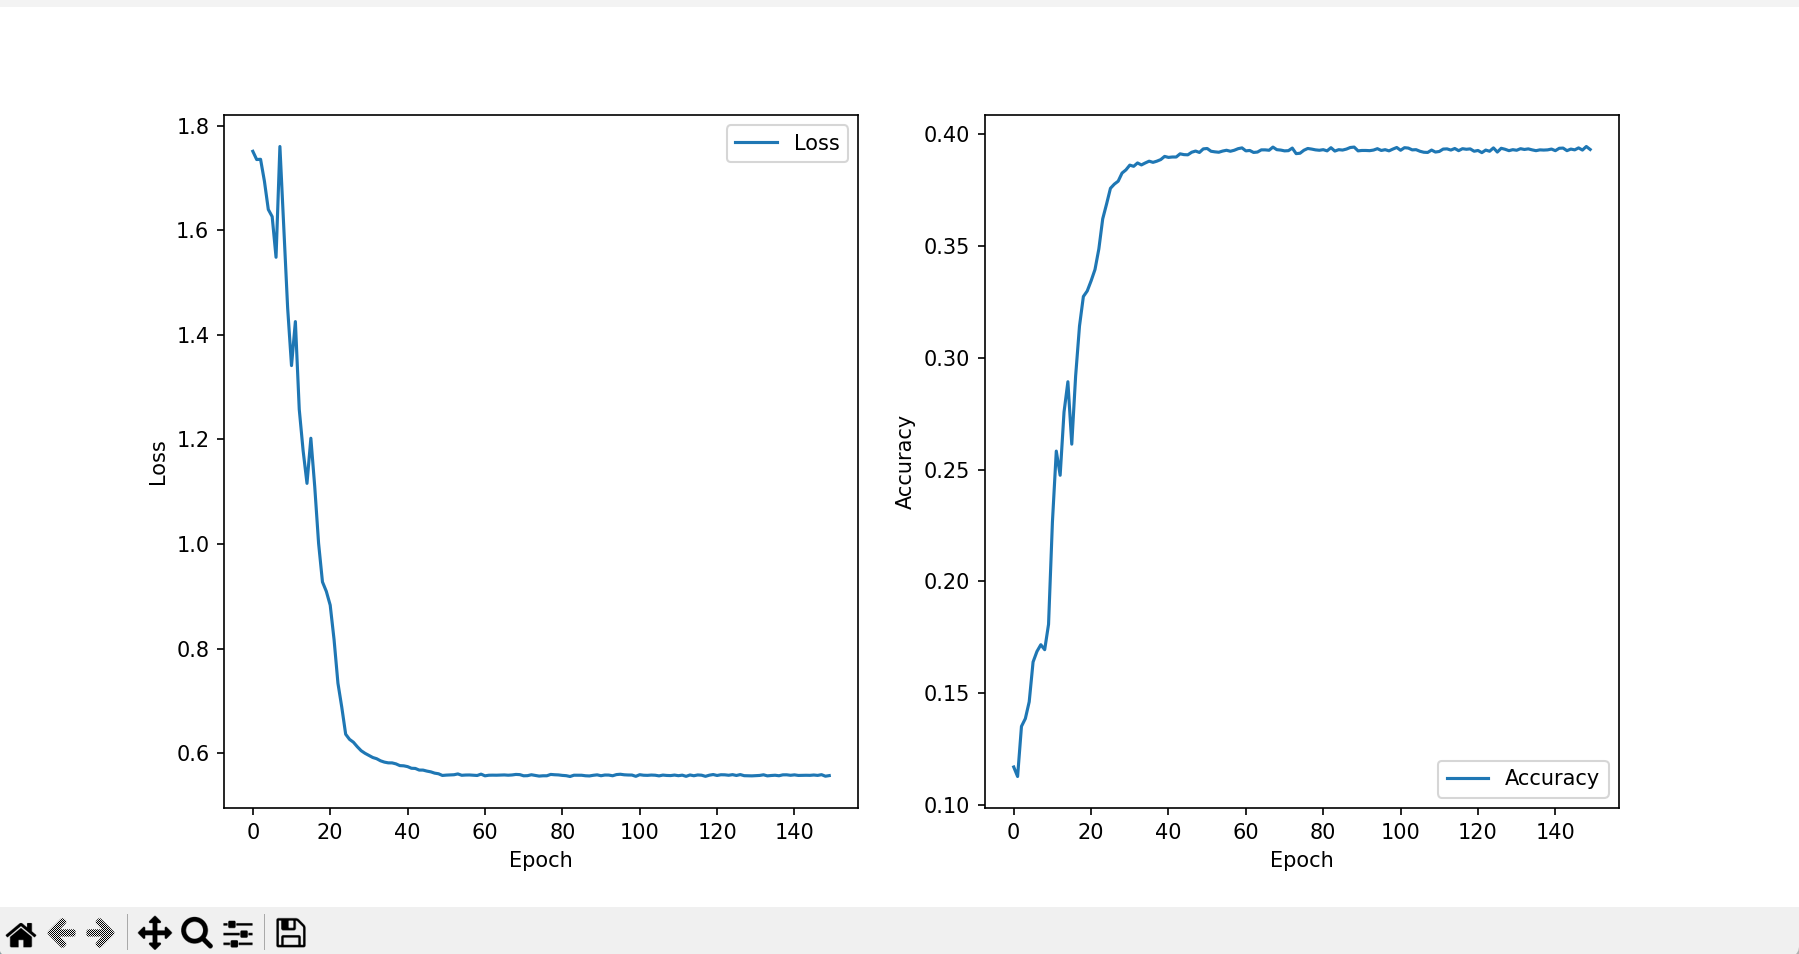
\includegraphics[scale=0.5]{graph/result4.png}
            \end{center}

            \subsubsection{结果分析}
            原因可能是因为,ground truth对应的函数关系非常复杂,这个模型学不到其全部的形式,
            也就无法做出正确的决策。另一方面尽管LSTM的设计目的是解决传统RNN的长程依赖问题,但在某些情况下,
            它仍然可能无法有效地捕捉到非常长的时间跨度内的依赖关系,例如对于本问题数据集的情感分析任务,
            每段对话的句子数量很多,但是可能在一段话内句子都存在上下文相关性。之所以Transformer的表现更好,
            就是因为Transformer最大的优势就是其满身的注意力机制。注意力机制更接近于人对序列的理解方式,
            能够彻底解决长记忆丢失问题,并且其并行能力远优于LSTM,
            在这种多模态情感分析的任务中显然更适合这种多层模型的训练任务。

            另一方面,其实尚未考虑到对说话人对象的嵌入,这一部分的信息并没有利用到LSTM中去。
            
        \subsection{Transformer\_Based模型}
            \subsubsection{训练结果}
            准确率:68\%-70\%

            F1\_Score:最高达到69.790648\%
            
            比赛成绩:由于数据集中给出了测试集的标签,导致比赛中部分队伍的正确率是1.0
            (根据工作人员表示,这些成绩会作废),但除去这些队伍,
            使用我们的Transformer\_Based模型的成绩是比赛中所有队伍最好的,反映了我们的模型设计是较好的。

            \begin{center}
                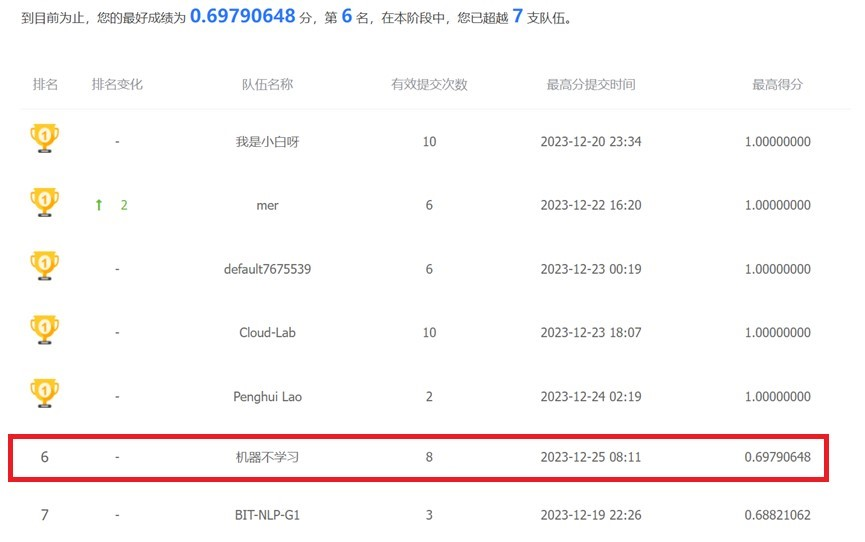
\includegraphics[scale=1]{graph/result5.jpg}
            \end{center}

            正确率和F1\_Score变化图:

            训练集和测试集正确率和F1\_Score变化图如下所示:

            \begin{center}
                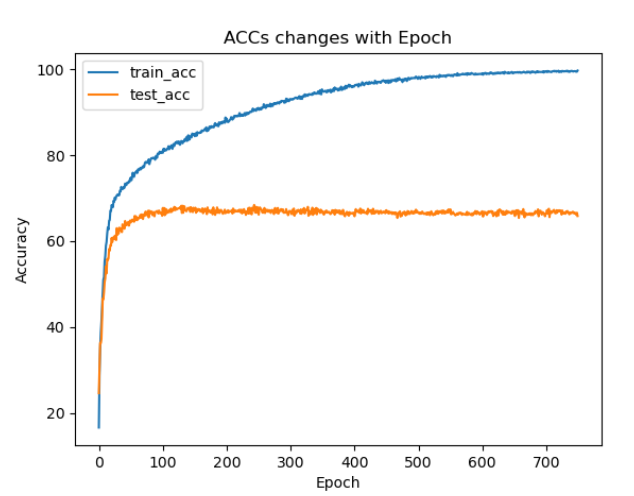
\includegraphics[scale=1]{graph/result5.png}\\
                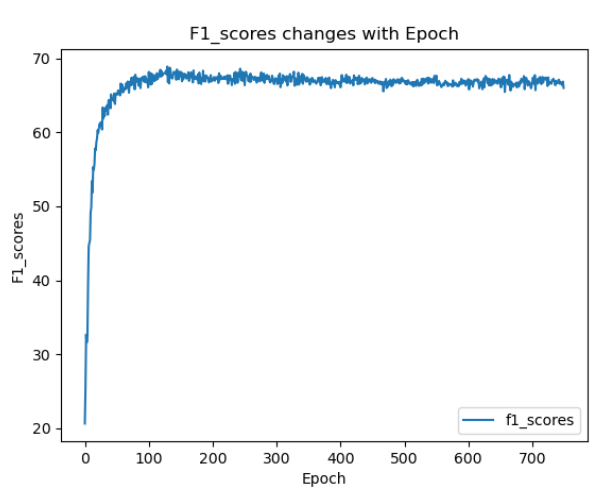
\includegraphics[scale = 0.9]{graph/result6.png}\\
            \end{center}

            可以看到,随着轮数的增多,训练集正确率不断上升,最终接近100\%,从训练集的loss可以看出,
            即使达到了750轮,loss也在不断下降。但测试集正确率在达到峰值70\%后,随后基本在68\%左右震荡,
            且在最后有略微下降的趋势,F1\_Score类似。
            
            可以看出,Transformer\_Based模型的收敛速度较快,且即使训练集正确率到达接近100\%,
            也没有出现较明显的过拟合现象,测试集正确率仍然较高。
            
            与之对比,当仅仅使用CNN和LSTM处理我们的数据集,正确率均不到30\%。为了得到其它方法的正确率,
            本组成员翻阅了IEMOCAP数据集有关的论文,得到的效果如下:

            \begin{center}
                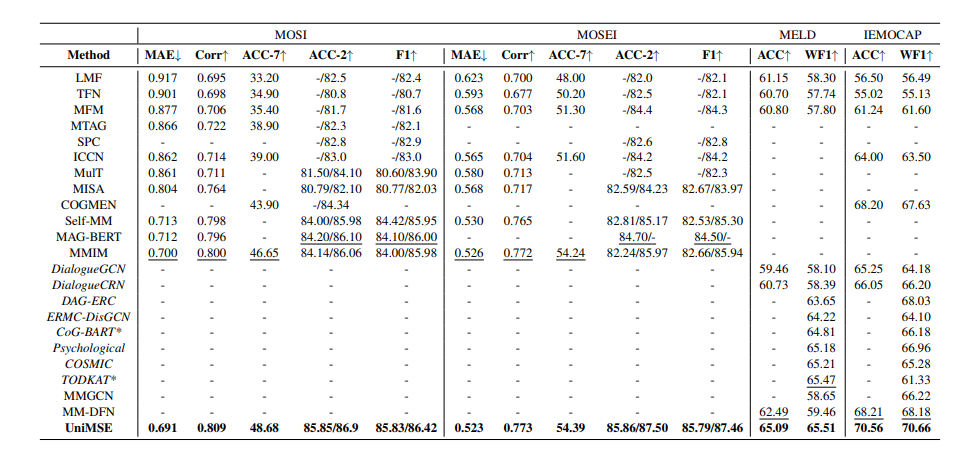
\includegraphics[scale=0.9]{graph/result7.png}
            \end{center}

            上面结果截图自\textit{ UniMSE: Towards Unified Multimodal Sentiment Analysis and Emotion Recognition. }论文,
            可以看到他们的方法在IEMOCAP上的正确率也仅仅达到70.56\%,而其它方法正确率均没有达到69\%,
            可以看出我们的正确率是很高的。
            
            综上,可以看到,Transformer\_Based模型的效果还是很出类拔萃的。

    \section{成员分工}
    \textbf{马迪峰:}完成决策树最初版模型的初稿和LSTM\_based模型的搭建,撰写机器学习汇报大纲。

    \textbf{盛子轩:}完成集成学习相关方法的总设计与代码编写,尝试采用决策树,逻辑斯蒂回归和随机森林等多种方法训练基学习器。

    \textbf{贾城昊:}完成Transformer\_Based模型的总设计与代码编写,预测结果的分析与绘制。参与了对\\LSTM的改良工作,使其能处理多个模态特征。

    \textbf{李金明:}参与对LSTM的调试工作,完善机器学习汇报。

    \section{参考文献}
    \begin{enumerate}
        \item [1]\href{https://bbs.huaweicloud.com/blogs/264134?utm_source=zhihu&utm_medium=bbs-ex&utm_campaign=ei&utm_content=content}{多模态学习综述-云社区-华为云 (huaweicloud.com)}
        \item [2]Vaswani, A., Shazeer, N., Parmar, N., Uszkoreit, J., Jones, L., Gomez, A. N., Kaiser, L., \& Polosukhin, I. (2017). Attention Is All You Need. arXiv preprint arXiv:1706.03762.
        \item [3]    Hu, G., Lin, T.-E., Zhao, Y., Lu, G., Wu, Y., \& Li, Y. (2022). "UniMSE: Towards Unified Multimodal Sentiment Analysis and Emotion Recognition." Accepted to EMNLP 2022 main conference. arXiv preprint arXiv:2211.11256.

        \item [4]Patamia, R. A., Santos, P. E., Acheampong, K. N., Ekong, F., Sarpong, K., \& Kun, S. (2023). "Multimodal Speech Emotion Recognition Using Modality-specific Self-Supervised Frameworks." arXiv preprint arXiv:2312.01568.

        \item [5]Ma, H., Wang, J., Lin, H., Zhang, B., Zhang, Y., \& Xu, B. (2023). "A Transformer-Based Model With Self-Distillation for Multimodal Emotion Recognition in Conversations." IEEE Transactions on Multimedia. doi:10.1109/TMM.2023.3271019.

        \item [6]Ahn, C.-S., Rajapakse, J. C., \& Rana, R. (2023). "Integrating Contrastive Learning into a Multitask Transformer Model for Effective Domain Adaptation." arXiv preprint arXiv:2310.04703.

        \item [7]Deep Learning []Ian Goodfellow , Yoshua Bengio,Aaron Courville.

    \end{enumerate}
    





   
    
    
    


\end{document}